\documentclass[14pt]{extarticle}
% \documentclass[14pt]{article}

% \usepackage[style=authoryear,maxbibnames=9,maxcitenames=2,uniquelist=false,backend=biber,doi=false,url=false]{biblatex}
% \addbibresource{$BIB} % bibtex location
% \renewcommand*{\nameyeardelim}{\addcomma\space} % have comma in parencite
\usepackage{natbib}

\usepackage{xcolor}
\usepackage{amsmath}
\newcommand{\tuple}[1]{ \langle #1 \rangle }
%\usepackage{automata}
\usepackage{times}
\usepackage{ltablex}
\usepackage{tasks}

%%%%%% Template
\usepackage{hyperref}
\hypersetup{colorlinks=true,allcolors=blue}

\usepackage{vmargin}
\setpapersize{USletter}
\setmarginsrb{1.0in}{1.0in}{1.0in}{0.6in}{0pt}{0pt}{0pt}{0.4in}

% HOW TO USE THE ABOVE:
%\setmarginsrb{leftmargin}{topmargin}{rightmargin}{bottommargin}{headheight}{headsep}{footheight}{footskip}
%\raggedbottom
% paragraphs indent & skip:
\parindent  0.3cm
\parskip    -0.01cm

\usepackage{tikz}
\usetikzlibrary{backgrounds}

% hyphenation:
% \hyphenpenalty=10000 % no hyphen
% \exhyphenpenalty=10000 % no hyphen
\sloppy

% notes-style paragraph spacing and indentation:
\usepackage{parskip}
\setlength{\parindent}{0cm}

% let derivations break across pages
\allowdisplaybreaks

\newcommand{\orange}[1]{\textcolor{orange}{#1}}
\newcommand{\blue}[1]{\textcolor{blue}{#1}}
\newcommand{\red}[1]{\textcolor{red}{#1}}
\newcommand{\freq}[1]{{\bf \sf F}(#1)}
\newcommand{\datafreq}[2]{{{\bf \sf F}_{#1}(#2)}}

\def\qqquad{\quad\qquad}
\def\qqqquad{\qquad\qquad}

%%%%%%%%%%%%%%%%%%%%%%%%%%%%%%%%%%%%%%%%%%%%%%%%%%%%%%%%%%%%%%%%%%%%%%%%%%%%%%%%
%%%%%%%%%%%%%%%%%%%%%%%%%%%%%%%%%%%%%%%%%%%%%%%%%%%%%%%%%%%%%%%%%%%%%%%%%%%%%%%%

% fill-in-blank question style, found in https://tex.stackexchange.com/a/505089

\usepackage{ifthen}
\usepackage{tocloft}
\usepackage{exercise}
% \usepackage{xcolor}

% Set the Show Answers Boolean
\newboolean{showAns}
\setboolean{showAns}{false}
\newcommand{\showAns}{\setboolean{showAns}{true}}

% The length of the Answer line
\newlength{\answerlength}
\newcommand{\anslen}[1]{\settowidth{\answerlength}{#1}}

% ans command that indicates space for an answer or shows the answer in red
\newcommand{\ans}[1]{\settowidth{\answerlength}{\hspace{2ex}#1\hspace{2ex}}%
    \ifthenelse{\boolean{showAns}}%
        {\textcolor{red}{\underline{\hspace{2ex}#1\hspace{2ex}}}}%
        {\underline{\hspace{\answerlength}}}}%

\newcommand{\details}[1]{\settowidth{\answerlength}{#1}%
    \ifthenelse{\boolean{showAns}}%
        {\\ \textcolor{blue}{#1}}%
        {}}%

% Formatting how multiple choices Questions are formated.
\settasks{label=(\Alph*), label-width=30pt}


% Some commands for the Exercise Question package
\renewcommand{\QuestionNB}{\Large\protect\textcircled{\small\bfseries\arabic{Question}}\ }
\renewcommand{\ExerciseHeader}{} %no header
\renewcommand{\QuestionBefore}{3ex} %Space above each Q
\setlength{\QuestionIndent}{8pt} % Indent after Q number


% To create the list of answers with tocloft...
\newcommand{\listanswername}{Answers}
\newlistof[Question]{answer}{Answers}{\listanswername}

% Creates a TOC for Answers
\newcounter{prevQ}
\newcommand{\answer}[1]{\refstepcounter{answer}%
\ans{#1}%
\ifnum\theQuestion=\theprevQ%
        \addcontentsline{Answers}{answer}{\protect\numberline{}#1}% don't include the Q number
        \else%
        \addcontentsline{Answers}{answer}{\protect\numberline{\theQuestion}#1}%
        \setcounter{prevQ}{\value{Question}}%
        \fi%
        }%

% \hyphenpenalty=10000 % no hyphen
% \exhyphenpenalty=10000 % no hyphen
\sloppy              % hyphen

\newcommand{\HRule}{\rule{\linewidth}{0.5mm}}
\newcommand{\Hrule}{\rule{\linewidth}{0.3mm}}

%tocloft formatting listofanswers
\renewcommand{\cftAnswerstitlefont}{\bfseries\large}
\renewcommand{\cftanswerdotsep}{\cftnodots}
\cftpagenumbersoff{answer}
\addtolength{\cftanswernumwidth}{10pt}

\makeatletter% since there's an at-sign (@) in the command name
\renewcommand{\@maketitle}{%
  \parindent=0pt% don't indent paragraphs in the title block
  \centering
  {\Large \bfseries\textsc{\@title}} \\
  \vspace{5pt}
  {\large \textit{\@author}} \\
  \HRule \\
  \vspace{1em}
}
\makeatother% resets the meaning of the at-sign (@)


\title{ECON 2002.01 Midterm Exam }
\author{Hui-Jun Chen}


%%%%%%%%%%%%%%%%%%%%%%%%%%%%%%%%%%%%%%%%%%%%%%%%%%%%%%%%%%%%%%%%%%%%%%%%%%%%%%%%
%%%%%%%%%%%%%%%%%%%%%%%%%%%%%%%%%%%%%%%%%%%%%%%%%%%%%%%%%%%%%%%%%%%%%%%%%%%%%%%%
\begin{document}

\maketitle

\showAns
\listofanswer


% \includegraphics[width=\textwidth]{../QuestionBankImage/}

\begin{Exercise}

\Question (OUP-U3-Q1) You currently work for 40 hours a week at wage rate of £12 an hour. Your free hours are defined as the number of hours not in work, which in this case is 24 hours × 7 days – 40 hours = 128 hours per week. Suppose that you are happy to keep your total weekly income constant. Then:
\answer{B}
\begin{tasks}(1)
    \task If your wage rate increases to £16 an hour, then your free time will increase by 6\%.
        \details{The current total weekly income is £12 × 40 hours = £480. At the wage rate of £16, you will only need to work for 480 /16 = 30 hours a week. This will increase your free time to 138 hours, which is an increase of (138 – 128) / 128 = 7.8\%.}
    \task To have 12.5\% more free time, your wage rate needs to increase by £8.
        \details{The current total weekly income is £12 × 40 hours = £480. 12.5\% extra free time means 128 hours × 1.125 = 144 hours of free time, or 24 hours of work. To keep your weekly income constant, your wage rate needs to increase to £480 / 24 = £20 an hour, which is an increase of £8.}
    \task Doubling the wage rate would decrease your working hours by a third.
        \details{The current total weekly income is £12 × 40 hours = £480. If the wage rate doubles to £24, your working hours fall to 480 /24 = 20 hours a week, i.e. it halves.}
    \task A wage cut of 25\% leaves you with only 100 hours of free time.
        \details{The current total weekly income is £12 × 40 hours = £480. A wage cut of 25\% means your new hourly wage is £12 × (1 – 0.25) = £9. To keep the weekly income constant you will have to work 480 ÷ 9 = 53 hours and 20 minutes, which leaves you with 114 hours and 40 minutes of free time.}
\end{tasks}

\newpage\Question (OUP-U3-Q9) The figure shows the indifference curves of a student for the two ‘goods’, free time and final grade. Based on this information, which of the following statements is correct?
\answer{A}
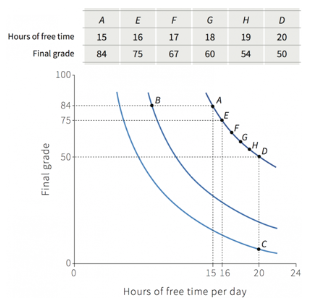
\includegraphics[width=\textwidth]{../QuestionBankImage/OUP-U3-Q9-01.png}
\begin{tasks}(1)
    \task At A, the student is willing to give up 34 grade points for five extra hours of free time.
        \details{This is true, as points A and D are on the same indifference curve.}
    \task A is the student’s most preferred choice as she would be attaining the highest grade.
        \details{The student is indifferent between A and all the other points on the same indifference curve i.e. E, F, G, H, and D.}
    \task The student strictly prefers a grade of 54 with 19 hours of free time to a grade of 67 with 18 hours of free time.
        \details{A grade of 54 with 19 hours of free time is point H. The student is indifferent between this point and point F, where she gets a grade of 67 with 17 hours of free time. She would therefore strictly prefer a grade of 67 with 18 hours of free time to H.}
    \task If at B the number of free hours is 10, then the student is 50\% happier at A than at B.
        \details{Higher indifference curves imply higher levels of utility, but the specific level of utility depends on the student’s relative preferences for both goods. It is not necessarily true that 50\% additional free time would make the student 50\% happier.}
\end{tasks}

\newpage\Question (OUP-U6-Q8)
Thomas earns £12 per hour in his current job and works 36 hours a week. He loves his job and puts in his maximum effort with no disutility. In fact, Thomas earns extra utility worth £3 per hour from camaraderie, status, and enjoyment of the job. If he loses this job Thomas has two choices. Either he is able to be self-employed, which earns him £7 an hour for 36 hours a week of work but also gives him disutility equivalent to £2 per hour, or he can be unemployed and receive an unemployment benefit of £150 per week. Thomas is expected to be able to find another job similar to his current one in 24 weeks. Then:
\answer{D}
\begin{tasks}(1)
    \task
Thomas’s next best option is to be unemployed.
        \details{
By being self-employed he will receive a benefit of (7 – 2) × 36 = £180 per week. This is higher than the unemployment benefit of £150 per week.
        }
    \task
The employment rent per hour is £8.
        \details{
The employment rent is (12 + 3) – (7 – 2) = £10 per hour.
        }
    \task
Thomas’s employment rent is £9,360.
        \details{
The employment rent is (12 + 3) – (7 – 2) = £10 per hour for 36 hours a week over the expected unemployment duration of 24 weeks i.e. 10 × 36 × 24 = £8,640.
        }
    \task
If Thomas chooses the self-employment option then his loss of employment rent is £8,640.
        \details{
		The loss of employment rent is the rent between the current job and self-employment. This is (12 + 3) – (7 – 2) = £10 per hour for 36 hours a week over the expected unemployment duration of 24 weeks i.e. 10 × 36 × 24 = £8,640.
        }
\end{tasks}

\newpage\Question (OUP-U6-Q16)
The figure depicts the efficiency wage equilibrium of a worker and a firm. Based on this information, which of the following statements is correct?
\answer{A}

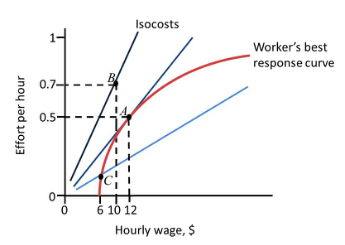
\includegraphics[width=\textwidth]{../QuestionBankImage/OUP-U6-Q15-01.png}
\begin{tasks}(1)
    \task
At A, given that the firm pays the hourly wage of \$12, the worker’s best response is to exert an effort of 0.5.
        \details{
This is true, by the definition of the worker’s best response curve.
        }
    \task
At A, given that the worker exerts an effort level of 0.5, the firm’s best response is to offer the hourly wage of \$12.
        \details{
The firm chooses to offer \$12 given the worker’s best response curve, rather than a particular effort level.	This is a sequential game where the firm chooses its action given the worker’s best responses to its actions.
        }
    \task
Therefore the worker receives no rent.
        \details{
The worker receives an employment rent because the efficiency wage is above her reservation wage. This wage level is required to induce her to put in some effort (of 0.5 in this case).
        }
    \task
The employer makes profits by coercing the worker to put in some effort.
        \details{
The employer’s power comes from the threat of job loss, which exists because the firm pays an efficiency wage above the worker’s reservation wage, giving the worker positive employment rents.
        }
\end{tasks}

\newpage\Question (ECO-U6-Q5)
Maria earns \$12 per hour in her current job and works 35 hours a week. Her disutility of effort is equivalent to a cost of \$2 per hour of work. If she loses her job, she will receive unemployment benefit equivalent to \$6 per hour. Additionally, being unemployed has psychological and social costs equivalent to \$1 per hour. Then:
\answer{D}
\begin{tasks}(1)
    \task
The employment rent per hour is \$3.
        \details{
Employment rent per hour = wage – unemployment benefit – disutility of effort + disutility of unemployment = 12 – 6 – 2 + 1 = \$5. This is the net hourly benefit of being employed compared with unemployment.
        }
    \task
Maria’s reservation wage is \$6 per hour.
        \details{
Maria’s reservation wage = unemployment benefit – disutility of unemployment = 6 – 1 = \$5. This is the wage at which Maria is just willing to forgo her unemployment benefits for a job (but it is not enough to make her put in effort!).
        }
    \task
Maria’s employment rent if she can get another job with the same wage rate after 44 weeks of being unemployed is \$6,160.
        \details{
Maria’s employment rent = \$5 (employment rent per hour) × 35 hours per week × 44 weeks = \$7,700.
        }
    \task
Maria’s employment rent if she can only get a job at a lower wage rate after 44 weeks of being unemployed is more than \$7,700.
        \details{
If she could get a job at the same wage after 44 weeks, Maria’s employment rent = \$5 (employment rent per hour) × 35 hours per week × 44 weeks = \$7,700. If the new job would have a lower wage, her employment rent would be higher than \$7,700.
        }
\end{tasks}

\newpage\Question (OUP-U7-Q8)
    The table represents market demand Q for a good at different prices P. The firm’s unit cost of production is £70. Based on this information, which of the following is correct?


\includegraphics[width=\textwidth]{../QuestionBankImage/OUP-U7-Q8-01.png}

\answer{C}
\begin{tasks}(1)
    \task
At Q = 200, the firm’s profit is £44,000.
        \details{At Q = 200, profit = (220 – 70) × 200 = £30,000. £44,000 is the total revenue.}
    \task
	The profit-maximising output is Q = 400.
        \details{At Q = 400, profit = (180 – 70) × 400 = £44,000. At Q = 500, profit = (160 – 70) × 500 = £45,000. Therefore Q = 400 is not the profit-maximising output.}
    \task
	The maximum profit that can be attained is £45,000.
        \details{The maximum profit is attained at Q = 500, where profit = (160 – 70) × 500 = £45,000. This can be checked by calculating profits at all P.}

    \task
	The minimum profit that can be attained is £0.
        \details{The firm makes a loss at Q = 1000, where the price is below the unit cost of production}
\end{tasks}

\newpage\Question
(ECO-U7-Q12) This figure shows the marginal cost and marginal revenue curves for Beautiful Cars. Which of the following statements is correct, based on the information shown?
\answer{D}

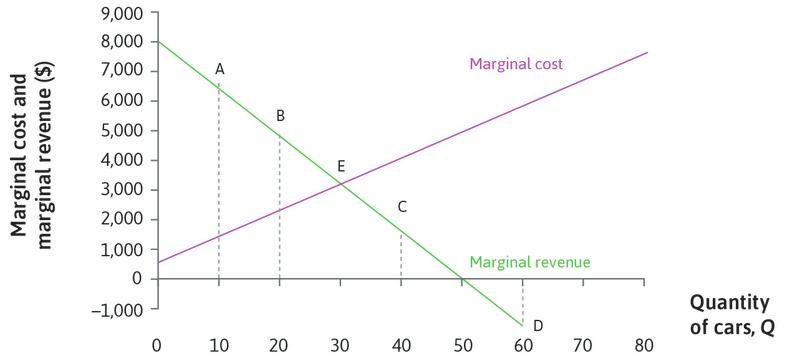
\includegraphics[width=\textwidth]{../QuestionBankImage/ECO-U7-Q12-01.jpg}
\begin{tasks}(1)
    \task
When Q = 40, the marginal cost is greater than the marginal revenue so the firm’s profit must be negative.
        \details{When Q = 40 the marginal cost is greater than the marginal revenue so the marginal profit is negative. This doesn’t mean that profit is negative.}
    \task
	Revenue is greater when Q = 10 than if Q = 20.
        \details{The marginal revenue is greater at Q = 10 than Q = 20. But because the marginal revenue is positive as output increases from 10 to 20, revenue is increasing: it is higher at Q = 20.}
    \task
	The firm would not choose to produce at point E because marginal profit is zero.
        \details{Marginal profit is zero at E. But this is the profit-maximizing point, so the firm will choose it.}
    \task
    	Profit is greater when Q = 20 than when Q = 10.
        \details{At all levels of output up to point E, marginal revenue is greater than marginal cost. So profit increases as output increases—it is higher at Q = 20 than Q = 10.	}
\end{tasks}

\newpage\Question (OUP-U9-Q22)
The figure describes the effect of immigration on unemployment in the labour market. The labour market equilibrium is at A and C before and after the influx of immigration, respectively. Based on this figure, which of the following statements is correct?
    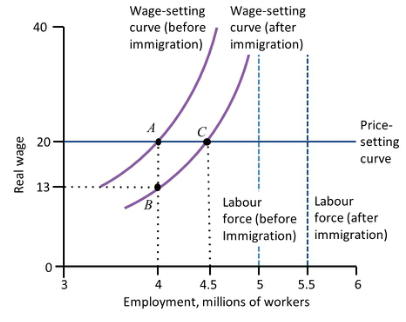
\includegraphics[width=\textwidth]{../QuestionBankImage/OUP-U9-Q22-01.png}

\answer{B}
\begin{tasks}(1)
    \task
All incumbent workers are unaffected while the labour market adjusts.
        \details{Workers face a temporary real wage cut from \$20 to \$13.}
    \task All incumbent workers are no worse off in the new equilibrium.
        \details{This is true as their employment status is unaffected and the real wage returns to \$20.}
    \task The unemployment rate is unchanged in the new equilibrium.
        \details{The number of unemployed is unchanged at 1 million before and after immigration. However the size of the labour force increases, so the unemployment rate drops after the immigration.}
    \task Firms claim a higher markup in the new equilibrium.
        \details{The average product of labour and the real wage are unchanged in the new equilibrium. Therefore the markup is also unchanged.	}
\end{tasks}

\newpage\Question (OUP-U10-Q12)
The diagram depicts Marco’s choice of consumptions in periods 1 and 2. He has \$100 worth of grain in period 1 and no income in period 2. Marco has two choices. In scheme 1, he can sell the grain that he does not consume and lend the money at 10\%. In scheme 2, he can invest the grain that he does not consume (e.g. planting as seed) for a return of 50\%. Which of the following statements is correct?
    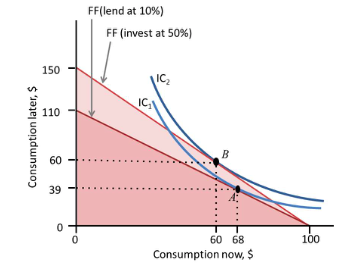
\includegraphics[width=\textwidth]{../QuestionBankImage/OUP-U10-Q12-01.png}
\answer{D}
\begin{tasks}(1)
    \task Marco is less impatient at B than at A.
        \details{The marginal rate of substitution is higher at B than at A. Therefore Marco is more impatient at B than at A.}
    \task Going from scheme 1 to scheme 2, the substitution and income effects have opposite effects on period 2 consumption.
        \details{A higher return means (i) it is more expensive to consume in period 1, and therefore the substitution effect is positive for period 2 consumption, and (ii) higher total income, which implies that the income effect is also positive for period 2 consumption.}
    \task Marco can do better than consumption choice B by investing all of his grain and consuming the output in period 2.
        \details{B is the point of tangency between the scheme 2 feasible frontier and the highest attainable indifference curve. Therefore he would be worse off at any other point on the feasible frontier, including at the ends.}
    \task Marco can do better than consumption choice B by investing all of his grain and borrowing against his period 2 output.
        \details{This shifts the feasible frontier out pivoted at the vertical axis, allowing Marco to attain higher indifference curves than $IC_2$.}
\end{tasks}

\newpage\Question (TEA-U10-Q2)
The following diagram depicts Julia’s choice of consumption now and consumption later (next period). She has no income now and an income of \$115 later. The current interest rate is 15\%. Based on this information, which of the following statements is correct?
    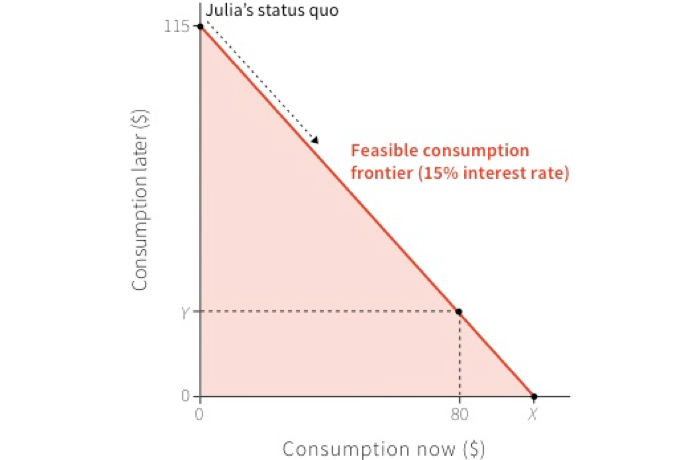
\includegraphics[width=\textwidth]{../QuestionBankImage/TEA-U10-Q2-01.png}
\answer{B}
\begin{tasks}(1)
    \task The maximum that Julia can borrow to spend now is \$91.
        \details{The maximum that Julia can borrow is $\$115/(1 + 0.15) = \$100$. This is the maximum that she can spend now.}
    \task If Julia borrows \$80 to spend now, she will have \$23 to spend later.
        \details{If Julia borrows \$80, she has to pay back $\$80 \times  1.15 = \$92$, so she will have \$115 - \$92 = \$23 to spend later.}
    \task The consumption choice of \$60 now and \$50 later is a feasible option.
        \details{When Julia borrows \$60, she has to pay back $\$60 \times  1.15 = \$69$, so she will have \$115 - \$69 = \$46 to spend later. Therefore the choice (60, 50) is not in her feasible set.}
    \task The feasible set will be smaller when the interest rate is 10\%.
        \details{When the interest rate falls, Julia’s feasible set will become larger: she will be able to borrow a maximum of \$115/(1 + 0.1) = \$104.5 to spend now.}
\end{tasks}

\newpage\Question (OUP-U3-Q17)
The figure shows a student’s feasible frontier and her indifference curves for her final exam grade and the hours of free time per day. Based on this information, which of the following statements is correct?
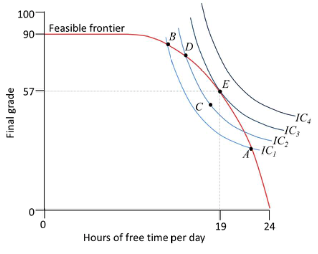
\includegraphics[width=\textwidth]{../QuestionBankImage/OUP-U3-Q17-01.png}
\answer{C}
\begin{tasks}(1)
    \task The student prefers D to C, as D is on the feasible frontier.
        \details{Both C and D are on the same indifference curve. So the student is indifferent between the two.}
    \task A or B may be chosen over C despite being on a lower indifference curve, as the student would never choose a point below the feasible frontier.
        \details{C is feasible and is strictly preferred to A and B, so A and B would never be chosen as the optimal choice.}
    \task Any points above $IC_3$ are strictly preferred to the student's final choice but are unattainable.
        \details{This is true. Points above $IC_3$ give higher utility but are not within her feasible set.}
    \task The student should try to attain as high a grade as possible.
        \details{The optimal choice balances the trade-off between grades and free time. By attempting to gain as high a grade as possible, the student is sacrificing expensive free time, the value of which would be higher than the value of extra grades.}
\end{tasks}




\newpage\Question (UCL-J17-Q4)
Suppose the utility function of an individual is given by: $U(x, y) = xy^2$.

\textit{Hint:} this question requires Calculus. If you are not comfortable with Calculus, use \underline{\href{https://www.wolframalpha.com/}{Wolfram Alpha}}!

\answer{C}
\begin{tasks}(1)
    \task This utility function implies that good $ y $ is preferred to good $ x $ so the bundle $(2, 1)$ is preferred to $(9, 0.5)$.
        \details{$(2, 1)$ gives a utility level of $ 2 $ and $(9, 0.5)$ gives a utility level of $2.25$, so $(9, 0.5)$ is preferred to $(2, 1)$.}
    \task The marginal rate of substitution between $ y $ and $ x $ is $MRS_{x, y} = \frac{2y}{x}$.
        \details{The marginal rate of substitution, in absolute value, is $\frac{y}{2x}$.}
    \task The marginal rate of substitution between $ y $ and $ x $ is decreasing in $ x $.
        \details{The marginal rate of substitution, in absolute value, is $\frac{y}{2x}$, so as $ x $ increases, the marginal rate of substitution decreases (in absolute value).}
    \task The marginal rate of substitution between $ y $ and $ x $ is decreasing in $ y $.
        \details{The marginal rate of substitution, in absolute value, is $\frac{y}{2x}$, so as $ y $ increases, the marginal rate of substitution increases.}
\end{tasks}



\newpage\Question (ECO-U3-Q6)
You are a taxi driver in Melbourne who earns \$50 for a day’s work. You have been offered a one-day ticket to the Australian Open for \$40. As a tennis fan, you value the experience at \$100. With this information, what can we say?
\answer{C}
\begin{tasks}(1)
    \task The opportunity cost of the day at the Open is \$40.
        \details{By going to the Open you are foregoing the opportunity of earning \$50 from taxi driving. This is your opportunity cost.}
    \task The economic cost of the day at the Open is \$40.
        \details{The economic cost is the sum of the actual price you pay plus the opportunity cost, which in this case is \$40 + \$50 = \$90.}
    \task The economic rent of the day at the Open is \$10.
        \details{The economic rent of an action is its benefit minus its economic cost (out-of-pocket plus opportunity costs). Therefore, the economic rent is $\$100 - \$40 - \$50 = \$10$.}
    \task You would have paid up to \$100 for the ticket.
        \details{The maximum price you would have paid for the ticket is the price at which your economic rent would be zero, which in this case is \$50.}
\end{tasks}



\newpage\Question (OUP-U6-Q15)
The figure depicts the efficiency wage equilibrium of a worker and a firm. According to this figure:
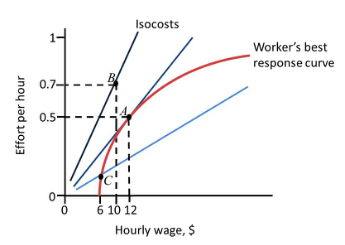
\includegraphics[width=\textwidth]{../QuestionBankImage/OUP-U6-Q15-01.png}
\answer{C}
\begin{tasks}(1)
    \task At C, the marginal rate of substitution (MRS) between higher wage cost and higher effort exceeds the marginal rate of transformation (MRT).
        \details{The MRS is the slope of the isocosts while the MRT is the slope of the worker’s best response curve. At C, the former is lower than the latter.}
    \task At B, the MRS is higher than the MRT.
        \details{B is not a feasible point. Therefore the MRT of higher wages into greater effort is not defined at this point.}
    \task The firm would maximise its profits by paying an hourly wage that is \$6 above the worker’s reservation wage.
        \details{The firm’s profit-maximising point is A, where it pays an efficiency wage of \$12 per hour. This is \$6 above the reservation wage of \$6.}
    \task The firm is able to increase its profits from those attained at A by inducing the worker to exert higher effort in return for a higher wage.
        \details{The units of effort per dollar of wage cost decrease to the right of A (the slope of the isocost that intersects the worker’s best response curve becomes flatter). Therefore the firm’s profit is decreasing to the right of A.}
\end{tasks}



\newpage\Question (TEA-U6-Q4)
The figure below depicts the effect of an increase in the unemployment benefit on the workers’ best response curve, when the unemployment rate is 12\%. Which of the following statements is correct following a rise in the unemployment benefit, ceteris paribus?
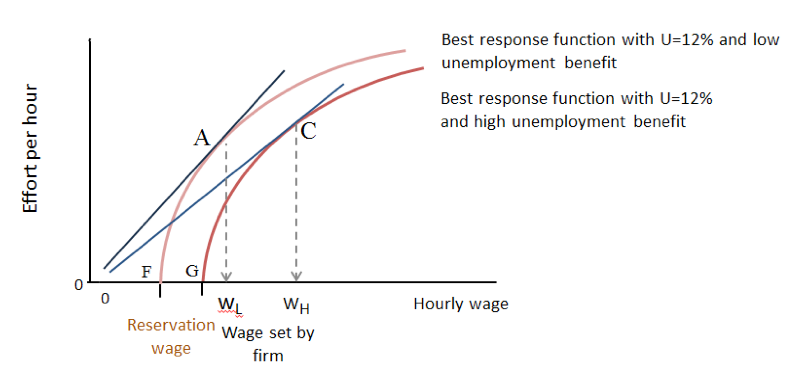
\includegraphics[width=\textwidth]{../QuestionBankImage/TEA-U6-Q4-01.png}
\answer{A}
\begin{tasks}(1)
    \task The firm’s profit level falls.
        \details{Higher unemployment benefits mean that the workers’ reservation wage will be higher, so the firm’s profit level falls.}
    \task The workers’ reservation wage falls.
        \details{Higher unemployment benefits increase the value of the workers’ reservation option, so their reservation wage will be higher.}
    \task The efficiency wage at any given level of employment falls.
        \details{The efficiency wage set by the firm rises from $W_L$ to $ W_H $, and this effect would be the same for all unemployment rates.}
    \task The firm sets a lower efficiency wage.
        \details{The efficiency wage set by the firm rises from $ W_L $ to $ W_H $, as depicted in the diagram.}
\end{tasks}



\newpage\Question (UCL-S17-Q6)
Clark and Oswald (2002) estimate that 'the average British person would need to be compensated £15,000 (\$22,500) per month after losing their job in order to be as happy as they were when they were employed.' Based on this information, which of the following statements is correct?

\textit{Hint:} this question is not asking you to find and read Clark and Oswald (2002). With merely knowledge on employment rent, you are able to answer this question.
\answer{C}
\begin{tasks}(1)
    \task This evidence favours the interpretation of unemployment as voluntary.
        \details{The converse is true: this evidence favours the interpretation of unemployment as involuntary.}
    \task This is less than the estimated loss of earnings of an average worker who became unemployed at that time.
        \details{The average worker earns much less than £15,000 per month, so this amount is considerably greater than the loss in earnings.}
    \task This evidence is an indicator that employment rents are non-negligible.
        \details{This evidence suggests that workers place a very high value on being employed, so employment rents are likely to be very large (and larger than the monetary earnings suggest).}
    \task This evidence shows that the motivation for worker to work with effort is the work ethic
        \details{The motivation in labor discipline model is fear of being fired.}
\end{tasks}



\newpage\Question (OUP-U6-Q14)

The figure depicts the isocost lines of a firm. Which of the following statements is correct?

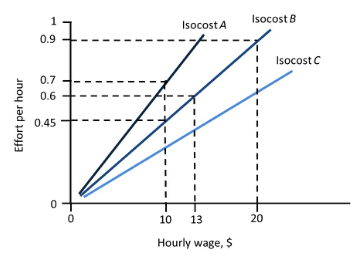
\includegraphics[width=\textwidth]{../QuestionBankImage/OUP-U6-Q14-01.png}

\answer{B}
\begin{tasks}(1)
    \task The cost of production is constant along an isocost line.
        \details{An isocost joins together a set of points that have the same ratio of effort to wages.}
    \task Isocost A has the lowest cost per unit of effort of the three isocosts.
        \details{The slope of the isocost lines is the units of effort per dollar of wage cost, which is the inverse of the cost per unit of effort. This is the lowest for isocost A.}
    \task The units of effort per dollar of wage cost for isocost B are 0.45.
        \details{The slope of the isocost lines is the units of effort per dollar of wage cost. For isocost B, this is 0.9/20 = 0.045.}
    \task For the hourly wage of \$12, the effort per hour is 0.8 on isocost A.
        \details{The slope of isocost A is 0.7/10 = 0.07. Therefore for hourly wage of \$12, the effort per hour would be $0.07 \times  12 = 0.84$.}
\end{tasks}



\newpage\Question (OUP-U6-Q10)
Consider an employee with a reservation wage of \$6 an hour. The employee chooses an effort level between zero and one. Which of the following statements regarding her best response curve is correct?
\answer{A}
\begin{tasks}(1)
    \task The best response curve describes the effort that the employee would choose for each level of the hourly wage.
        \details{This is the definition of the employee’s best response curve.}
    \task The best response curve is upward-sloping and convex.
        \details{The higher the wage level, the higher the employment rent and therefore the higher the effort exerted (more to lose if fired). Therefore the best response curve is upward-sloping. However the higher the wage level, the higher the additional wage required to induce an additional unit of effort (diminishing marginal returns), and therefore the curve is concave.}
    \task The curve crosses the horizontal axis at the origin.
        \details{The curve crosses the horizontal axis at the reservation wage of \$6.}
    \task The average effort per hour is increasing in wages.
        \details{The average effort per hour is the slope of the ray from the horizontal axis intercept to the best response curve. For a concave curve, this is decreasing in wages.}
\end{tasks}



\newpage\Question (OUP-U7-Q14)
The following table shows the total cost (TC), average cost (AC), and marginal cost (MC) of a firm for different outputs Q. Which of the following numbers correctly fills in the corresponding letter in the table?

\textit{Hint:} All three rows, $ TC $, $ AC $ and $ MC $ are continuous lines with $ Q $ on the $ x $-axis.

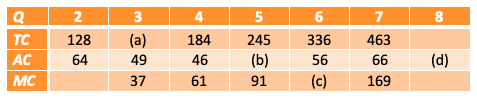
\includegraphics[width=\textwidth]{../QuestionBankImage/OUP-U7-Q14-01.png}
\answer{D}
\begin{tasks}(1)
    \task $156$
        \details{$TC = AC \times  Q = 49 × 3 = 147$.}
    \task $ 43 $
        \details{$AC = \frac{TC}{Q} = \frac{245}{5} = 49$.}
    \task $ 130 $
        \details{$MC_6 = TC_7 - TC_6 = 463 - 336 = 127.$}
    \task $ 79 $
        \details{$TC_8 = TC_7 + MC_7 = 463 + 169 = 632.$ Then $AC_8 = \frac{TC_8}{Q_8} = \frac{632}{8} = 79$.}
\end{tasks}



\newpage\Question (OUP-U7-Q25)
Which of the following statements regarding the cost structure of the film (movie) industry is correct?
\answer{D}
\begin{tasks}(1)
    \task The marginal cost of producing additional copies of a film is high.
        \details{The marginal cost of producing additional copies of a film is typically low: once the first copy is produced, subsequent copies are cheap to reproduce.}
    \task The price is above marginal cost due to lack of substitutes.
        \details{The film industry is quite competitive as consumers have many close substitutes. The price is above marginal cost because of the high fixed costs of hiring actors, technicians, a director, purchasing rights to the script, and advertising (known as first copy costs).}
    \task Industry regulators should cap the price of a DVD at its marginal cost.
        \details{Due to the existence of fixed costs (the first copy costs), the average cost is higher than the marginal cost. Capping the price at marginal cost would lead to firms being unable to cover their fixed costs.}
    \task The quantity sold in the film industry is inefficient.
        \details{The fact that the price is above marginal cost means that there is market failure, as there are some potential buyers whose willingness to pay exceeds the marginal cost but falls short of the market price. This creates a deadweight loss.}
\end{tasks}




\newpage\Question (UCL-S16-Q4)
Demand faced by a monopolist is $Q = 20 – 0.5P$. Her marginal cost is $ 10 $. Based on this information we can say that:
\answer{C}
\begin{tasks}(1)
    \task The optimal production of the monopolist is Q = 15.
        \details{The monopolist will produce until $MR = MC$. From the demand function, we find that $P = 40 - 2Q$. Therefore, revenue R is $R = Q \times  P = 40Q - 2Q^2$. Marginal revenue MR is: $\frac{dR}{dQ} = MR = 40 - 4Q$. Because $MR = MC$, then $40 - 4Q = 10$ which implies that Q* = 7.5. So the monopolist will produce 7.5 units.}
    \task The price charged by the monopolist is equal to her marginal cost.
        \details{This would be true in case of perfect competition. In this case, the price is obtained through the inverse demand function: $P* = 40 - 2Q* = 40 - 2 \times  7.5 = 25$.}
    \task The deadweight loss associated with the monopolist’s choice of price is less than the product of the difference between her price and marginal cost, multiplied by her optimal quantity.
        \details{The deadweight loss (DWL) associated with the monopolist's choice is DWL = $(1/2) \times  ((25 - 10) x (15 - 7.5)) = 56.25$. The product of the difference between her price and marginal cost multiplied by her optimal quantity is given by $(25 - 10) \times  7.5 = 112.5$.}
    \task If instead of a monopolist, the market is under perfect competition, then the optimal production of this tiny firm would be Q = 7.5 .
        \details{The tiny firm under perfect competition will produce until $P = MC$. From the demand function, we find that $P = 40 - 2Q$. Therefore,  $40 - 2Q = 10$ which implies that $Q* = 15$. So the tiny firm will produce 15 units.}
\end{tasks}



\newpage\Question (OUP-U9-Q4)
The figures depict the wage-setting curve and how it is derived using the best response function of the employees and the isocost lines for effort of the employers. $ U_1 $ and $ U_2 $ are unemployment rates. Which of the following statements is correct?

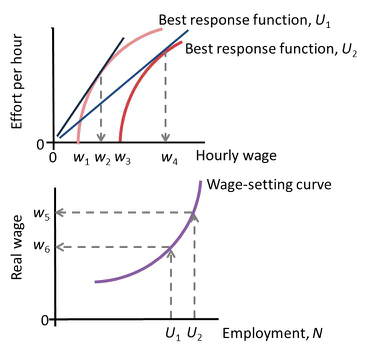
\includegraphics[width=\textwidth]{../QuestionBankImage/OUP-U9-Q4-01.png}

\answer{D}
\begin{tasks}(1)
    \task $ w_2 $ is the reservation wage when the unemployment rate is $ U_1 $.
        \details{$ w_1 $ is the reservation wage when the unemployment rate is $ U_1 $.}
    \task $w_5 = w_3$.
        \details{$ w_5 $ in the second diagram is the wage that maximises the effort per hour when the unemployment rate is $ U_2 $. This equals $ w_4 $ in the first diagram.}
    \task $ U_1 < U_2 $.
        \details{In the first diagram, $ U_1 $ requires a lower wage level to attain the optimal level of effort than $ U_2 $. In the second diagram, $ U_1 $ corresponds to the lower employment rate. In either case, the unemployment rate $U_1 > U_2$.}
    \task $ w_5 $ is the Nash equilibrium wage when the unemployment rate is $ U_2 $.
        \details{This is correct. At unemployment rate $ U_2 $, wage $ w_5 $ is the result of both employers and employees doing the best they can in setting wages and responding to the wage with a given amount of effort, respectively}
\end{tasks}



\newpage\Question (OUP-U9-Q21)
The figure depicts a labour market. Now consider an inflow of half a million immigrant workers who are all looking for employment (rather than intending to start up a business). Which of the following statements is correct?

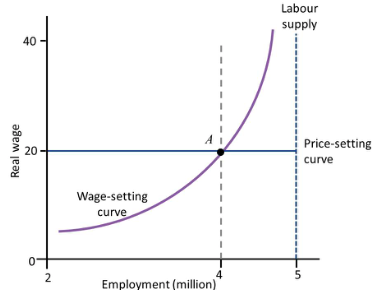
\includegraphics[width=\textwidth]{../QuestionBankImage/OUP-U9-Q21-01.png}

\answer{C}
\begin{tasks}(1)
    \task Unemployment doubles initially.
        \details{Before the labour supply increase there are 1 million unemployed. With the extra half a million workers joining the labour supply, unemployment initially rises to 1.5 million, which is a 50\% increase.}
    \task The wage-setting curve temporarily shifts down.
        \details{With higher unemployment rate, workers’ economic rent increases. This means that firms are able to pay a lower wage and can still induce workers to exert effort. This results in a permanent downward shift of the wage-setting curve.}
    \task The firms’ marginal cost of production is temporarily reduced.
        \details{With the downward shift of the wage-setting curve, the firms’ marginal cost of production initially falls. This induces them to employ more workers, moving up the wage-setting curve, thus raising the marginal cost again.}
    \task All immigrants find work.
        \details{At the higher labour supply, the unemployment level required for the workers to be just incentivised to exert effort may be higher than before, in which case the unemployment level is increased.}
\end{tasks}



\newpage\Question (ECO-U9-Q11)
Figure 9.20 depicts the effect of union wage-setting. What can we conclude from this figure?

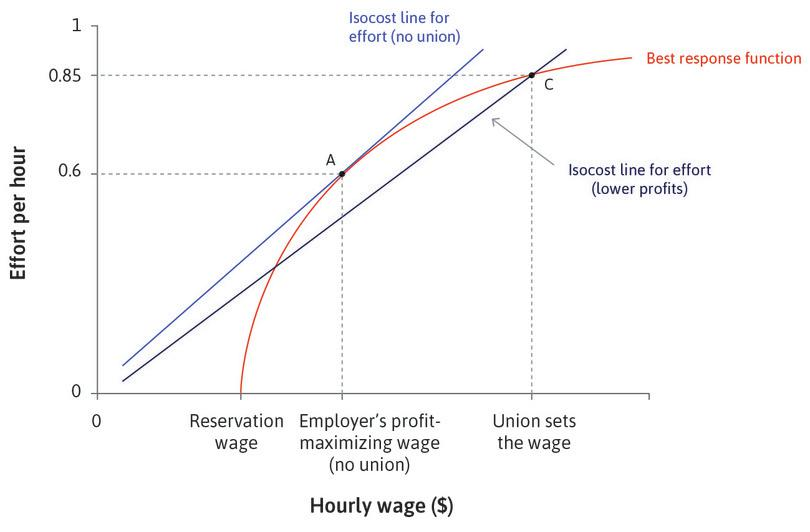
\includegraphics[width=\textwidth]{../QuestionBankImage/ECO-U9-Q11-01.jpg}

\answer{B}
\begin{tasks}(1)
    \task Compared to A, at C the effort per hour is higher and therefore the firm’s profit is higher.
        \details{The isocost line is flatter through C than through A. This means that the firm receives less effort from workers for each dollar spent on wages. Therefore the firm’s profit is lower at C.}
    \task The resulting bargained wage-setting curve will be above the wage-setting curve with no union.
        \details{Due to the union effect, employees need to be paid a higher wage to work hard, compared to when there is no union. This shifts the wage-setting curve higher.}
    \task The effect of a strong union will always be to increase unemployment.
        \details{If the employees reciprocate (for example when they have a lower disutility of effort) and there is a ‘union voice effect’, then this has an effect of shifting the wage-setting curve downward. If this more than offsets the wage bargaining effect that shifts the wage-setting curve up, then there will be an overall decrease in unemployment.}
    \task Under union wage-setting, the firm is still setting the wage that maximizes its profits.
        \details{Unlike at A, at C the firm is not producing at the point of tangency between the isocost line and the best response curve. Therefore it is no longer setting the profit-maximizing wage level.}
\end{tasks}



\newpage\Question (OUP-U10-Q3)
Ms. Moneypenny’s wealth depreciates at £5,000 a year. Her net annual income is £25,000. She will spend 40\% of this net income on an extension on the house, another 40\% on general consumption and save the remaining 20\% in a pension fund. The tax rate is 40\%. Based on this information, which of the following statements is correct?
\answer{B}
\begin{tasks}(1)
    \task Her annual disposable income is £20,000.
        \details{Net income = disposable income – depreciation. Therefore disposable income = net income + depreciation = 25,000 + 5,000 = £30,000.}
    \task Her before-tax income is £50,000.
        \details{Disposable income = before-tax income × (1 – t), where t is the tax rate. The disposable income = net income + depreciation = 25,000 + 5,000 = £30,000. Therefore before-tax income = disposable income/(1 – t) = 30,000/0.6 = £50,000.}
    \task Her investment is £5,000.
        \details{She saves 25,000 × 0.2 = £5,000 in the pension fund. However in economics, investment is expenditure on capital goods rather than in financial assets. Therefore her expenditure on the extension is considered as an investment, which is 25,000 × 0.4 = £10,000.}
    \task She pays a tax of £12,000.
        \details{Tax = before-tax income × tax rate. Before-tax income is £50,000. Therefore tax = 50,000 × 0.4 = £20,000.}
\end{tasks}




\newpage\Question (OUP-U10-Q5)
Consider Esther’s intertemporal choice of consumption (c1, c2), where c1 and c2 are the consumption level in periods 1 (horizontal axis variable) and 2 (vertical axis variable), respectively. You are given that her preferences exhibit diminishing marginal returns to consumption. Which of the following statements is correct?

\textit{Hint:} Usually indifference is convex.

\answer{D}
\begin{tasks}(1)
    \task If Esther is willing to substitute €1 of c1 for €5 of c2 when c1 is €5, then she would be willing to substitute €1 of c1 for more than €5 of c2 if c1 was €10.
        \details{Due to diminishing marginal returns to consumption, c1 is worth relatively less compared with c2 when c1 is higher. Therefore Esther would be willing to substitute €1 of c1 for less than €5 of c2 if c1 is €10.}
    \task Esther’s indifference curves are concave.
        \details{Esther’s indifference curves are convex (bowed toward the origin).}
    \task Esther’s marginal rate of substitution is decreasing in c2.
        \details{Esther’s marginal rate of substitution (absolute value of the slope of her indifference curve) is decreasing in c1 and increasing in c2.}
    \task Esther prefers similar amounts of c1 and c2 compared to the extreme cases of consuming all of her income as c1 or c2.
        \details{Diminishing marginal returns to consumption means that Esther prefers to smooth her consumption between the periods.}
\end{tasks}

\newpage\Question (OUP-U10-Q10)

The diagram depicts Marco’s choice of consumptions in periods 1 and 2. He has \$100 worth of grain in period 1 and no income in period 2. Marco has two choices. In scheme 1, he can store the grain that he does not consume in period 1. This results in a loss of 20\% of the grain due to pests and rotting. In scheme 2, he can sell the grain that he does not consume and lend the money at 10\%. Which of the following statements is correct?

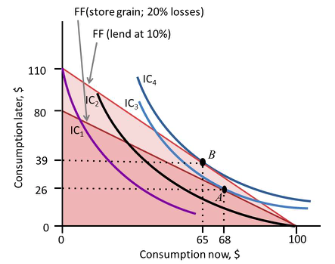
\includegraphics[width=\textwidth]{../QuestionBankImage/OUP-U10-Q10-01.png}

\answer{B}
\begin{tasks}(1)
    \task $ IC_1 $ is Marco’s reservation indifference curve.
        \details{$ IC_2 $ is Marco’s reservation indifference curve, because he has an endowment in period 1 and not in period 2.}
    \task Storing some of the grain is beneficial for Marco, despite the loss due to pests and rotting.
        \details{By storing some of the grain, Marco can move to an indifference curve (e.g. $ IC_3 $) above his reservation indifference curve $ IC_2 $.}
    \task At A, Marco loses \$26 worth of grain to pests and rotting.
        \details{At A, \$26 is how much Marco can consume in period 2. The loss to pests and rotting is 100 – (68 + 26) = \$6.}
    \task As Marco can earn 10\% interest with scheme 2, his best option is to sell all of his grain and lend.
        \details{This leads to Marco not consuming in period 1 at all and consuming \$110 in period 2. This places him on indifference curve $ IC_1 $, which is even lower than his reservation indifference curve $ IC_2 $.}
\end{tasks}



\newpage\Question (OUP-U10-Q22)
Which of the following statements is correct?
\answer{A}
\begin{tasks}(1)
    \task A bank is insolvent if the value of its liabilities exceeds the value of its assets.
        \details{In this case the net worth is negative, making the bank insolvent.}
    \task The net worth of a bank belongs to its employees.
        \details{A bank’s net worth is its equity. This belongs to its shareholders or its owners.}
    \task A loan is secured if it is default-free.
        \details{A loan is secured if the borrower has provided collateral. The borrower can still default on the loan.}
    \task The more a bank holds in cash and reserves, the higher its profits.
        \details{Larger cash and reserves means that the bank is more able to meet the demand by depositors for funds. However holding cash and reserves has an opportunity cost, as they could instead be lent out in the money market to earn interest.}
\end{tasks}



\newpage\Question (TEA-U10-Q7)
Which of the following statements about the banking system is correct?
\answer{A}
\begin{tasks}(1)
    \task The policy rate is the rate at which the central bank lends to commercial banks.
        \details{The policy rate is the interest rate set by the central bank, which applies to banks that borrow base money from each other, and from the central bank.}
    \task The policy rate is determined by the supply and demand of the money market.
        \details{The policy rate is determined entirely by supply; the central bank commits itself to supply any amount of money at that rate.}
    \task The bank lending rate is the rate at which the central bank lends to commercial banks.
        \details{The bank lending rate is the average interest rate charged by commercial banks to firms and households.}
    \task The spread (markup) represents how the central bank’s money is distributed amongst the commercial banks.
        \details{The spread (markup) is the difference between the bank lending rate and the policy rate.}
\end{tasks}


\newpage\Question (OUP-U10-Q25)
In an economy with a population of 100, there are 75 farmers and 25 lenders. The farmers use the funds to finance the planting and tending of their crops. The rate of profit for the harvest is 10\%, while the interest rate charged is 6\%. Compare the following two cases.

\begin{itemize}
    \item Case A: All farmers are able to borrow.
    \item Case B: 40 farmers are credit-excluded.
\end{itemize}

The Lorenz curves for the two cases are depicted in the figure. Based on this information, which of the following statements is correct?

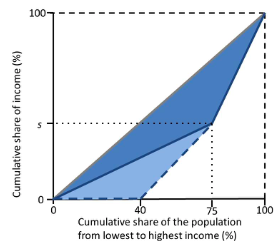
\includegraphics[width=\textwidth]{../QuestionBankImage/OUP-U10-Q25-01.png}

\answer{D}
\begin{tasks}(1)
    \task The lenders’ share of the total income is 40\%.
        \details{The lenders’ share is the interest rate charged / the rate of profit = 6 / 10 = 60\%.}
    \task s = 60\%.
        \details{s is the farmers’ share of the total income. This is 1 – interest rate charged / the rate of profit = 1 – (6 / 10) = 40\%.}
    \task The Gini coefficient for Case A is 0.4.
        \details{The Gini coefficient for Case A is 0.35.}
    \task The Gini coefficient for Case B is 0.16 higher than the coefficient for Case A.
        \details{The Gini coefficient is 0.35 for Case A and 0.51 for Case B. Therefore the latter is 0.16 higher than the former.}
\end{tasks}


\end{Exercise}

\end{document}
